% ============================================================
% 讲义 — 初升高衔接 · 锐角三角函数巩固
% 编译命令：xelatex -interaction=nonstopmode 衔接5_锐角三角函数巩固.tex
% ============================================================
\documentclass[12pt, a4paper]{ctexart}
\usepackage[margin=2.2cm]{geometry}
\usepackage{amsmath, amssymb}
\usepackage{enumitem}
\usepackage{tcolorbox}
\usepackage{booktabs}
\usepackage{array}
\usepackage{fancyhdr}
\usepackage{xcolor}
\usepackage{tikz}
\usetikzlibrary{calc}
\usepackage{hyperref}
\usepackage{graphicx}
\usepackage{multirow}
\usepackage{pgfplots}
\pgfplotsset{compat=1.18}

% 颜色定义
\definecolor{mainblue}{RGB}{41, 98, 168}
\definecolor{lightblue}{RGB}{230, 240, 255}
\definecolor{tipgreen}{RGB}{34, 139, 87}
\definecolor{lightgreen}{RGB}{235, 250, 240}
\definecolor{warnred}{RGB}{200, 50, 50}
\definecolor{lightred}{RGB}{255, 240, 240}
\definecolor{examorange}{RGB}{210, 120, 20}
\definecolor{lightorange}{RGB}{255, 248, 235}
\definecolor{apppurple}{RGB}{120, 60, 170}
\definecolor{lightpurple}{RGB}{245, 238, 255}

% 页眉页脚
\pagestyle{fancy}
\fancyhf{}
\fancyhead[L]{\small\textcolor{mainblue}{\textbf{初升高衔接 · 锐角三角函数}}}
\fancyhead[R]{\small\textcolor{mainblue}{初升高衔接讲义}}
\fancyfoot[C]{\small —\ \thepage\ —}
\renewcommand{\headrulewidth}{0.6pt}
\renewcommand{\headrule}{\hbox to\headwidth{\color{mainblue}\leaders\hrule height \headrulewidth\hfill}}
\renewcommand{\footrulewidth}{0pt}

% tcolorbox 样式
\newtcolorbox{knowledgebox}[1][]{%
  colback=lightblue, colframe=mainblue,
  fonttitle=\bfseries\large, title=#1,
  arc=3mm, boxrule=0.8pt,
  left=8pt, right=8pt, top=6pt, bottom=6pt
}

\newtcolorbox{tipbox}[1][]{%
  colback=lightgreen, colframe=tipgreen,
  fonttitle=\bfseries, title=#1,
  arc=2mm, boxrule=0.6pt,
  left=6pt, right=6pt, top=4pt, bottom=4pt
}

\newtcolorbox{warnbox}[1][]{%
  colback=lightred, colframe=warnred,
  fonttitle=\bfseries, title=#1,
  arc=2mm, boxrule=0.6pt,
  left=6pt, right=6pt, top=4pt, bottom=4pt
}

\newtcolorbox{examplebox}[1][]{%
  colback=lightorange, colframe=examorange,
  fonttitle=\bfseries, title=#1,
  arc=3mm, boxrule=0.8pt,
  left=8pt, right=8pt, top=6pt, bottom=6pt
}

\newtcolorbox{appbox}[1][]{%
  colback=lightpurple, colframe=apppurple,
  fonttitle=\bfseries, title=#1,
  arc=3mm, boxrule=0.8pt,
  left=8pt, right=8pt, top=6pt, bottom=6pt
}

\setCJKmainfont{Hiragino Sans GB}
\setCJKsansfont{Heiti SC}

\begin{document}

% ============ 标题页 ============
\begin{center}
{\Huge\bfseries\textcolor{mainblue}{锐角三角函数巩固}}\\[12pt]
{\Large\textcolor{gray}{初升高衔接讲义}}\\[8pt]
\rule{0.6\textwidth}{1pt}\\[8pt]
{\normalsize 目标：夯实初中三角函数基础\quad |\quad 为高中三角函数做好准备}
\end{center}
\vspace{10pt}

% ============================================================
%  第一部分：知识点讲解
% ============================================================
\section*{\textcolor{mainblue}{一、知识点讲解}}

% ------- 1.1 三角函数的定义 -------
\subsection*{1.1\quad 锐角三角函数的定义}

\begin{knowledgebox}[核心概念]
在直角三角形中，$\angle C=90°$，设 $\angle A$ 的对边为 $a$，邻边为 $b$，斜边为 $c$。

\medskip
\begin{center}
\begin{tikzpicture}[scale=1.3]
  \coordinate (C) at (0,0);
  \coordinate (A) at (0,4);
  \coordinate (B) at (5,0);
  % 画直角三角形
  \draw[thick,mainblue] (A)--(B)--(C)--cycle;
  % 直角标记
  \filldraw[mainblue!30] (0,0.4) rectangle (0.4,0);
  \draw[thick,mainblue] (0,0.4)--(0.4,0.4)--(0.4,0);
  % 标注顶点
  \node[above left] at (A) {$A$};
  \node[below right] at (B) {$B$};
  \node[below left] at (C) {$C$};
  % 标注边
  \node[left] at ($(A)!0.5!(C)$) {$a$（对边）};
  \node[below] at ($(B)!0.5!(C)$) {$b$（邻边）};
  \node[above right,shift={(0.15,-0.15)}] at ($(A)!0.5!(B)$) {$c$（斜边）};
  % 标注角A
  \draw[red,thick] (A) ++(-0.5,-0.05) arc(-175:-120:0.5);
  \node at ($(A)+(-148:0.85)$) {\small $\angle A$};
\end{tikzpicture}
\end{center}

\medskip
\begin{itemize}[nosep, leftmargin=2em]
  \item \textbf{正弦}：$\sin A = \dfrac{\angle A\;\text{的对边}}{\text{斜边}} = \dfrac{a}{c}$
  \item \textbf{余弦}：$\cos A = \dfrac{\angle A\;\text{的邻边}}{\text{斜边}} = \dfrac{b}{c}$
  \item \textbf{正切}：$\tan A = \dfrac{\angle A\;\text{的对边}}{\angle A\;\text{的邻边}} = \dfrac{a}{b}$
\end{itemize}

\medskip
\textbf{记忆口诀：}正弦对斜、余弦邻斜、正切对邻。简记为\textbf{"对弦斜，邻弦斜，对切邻"}。
\end{knowledgebox}

\begin{warnbox}[易错提醒]
\begin{enumerate}[nosep, leftmargin=1.5em]
  \item $\sin A$、$\cos A$、$\tan A$ 是一个\textbf{整体符号}，不是 $\sin\times A$。
  \item "对边"和"邻边"是\textbf{相对于所讨论的角}而言的。同一个三角形中，$\angle A$ 的对边是 $\angle B$ 的邻边！
  \item $\sin A$ 和 $\cos A$ 的值在 $0$ 到 $1$ 之间（$A$ 为锐角），但 $\tan A$ 可以大于 $1$。
  \item 三角函数值只与\textbf{角的大小}有关，与三角形的大小无关。
\end{enumerate}
\end{warnbox}

% ------- 1.2 特殊角的三角函数值 -------
\subsection*{1.2\quad 特殊角的三角函数值（必须熟记！）}

\begin{knowledgebox}[特殊角的三角函数值]

\textbf{一、$45°$ 角——等腰直角三角形}

\begin{center}
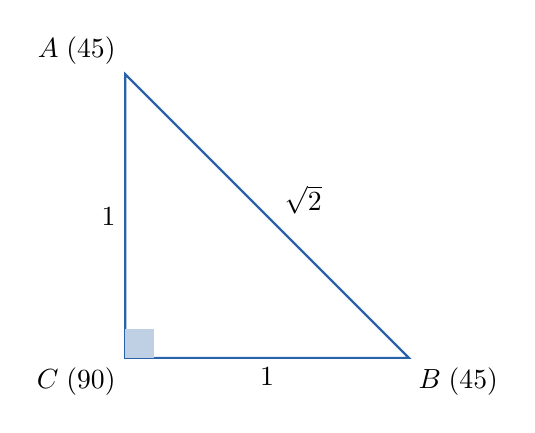
\begin{tikzpicture}[scale=1.2]
  \coordinate (C) at (0,0);
  \coordinate (A) at (0,3);
  \coordinate (B) at (3,0);
  \draw[thick,mainblue] (A)--(B)--(C)--cycle;
  \filldraw[mainblue!30] (0,0.3) rectangle (0.3,0);
  \node[above left] at (A) {$A\;(45°)$};
  \node[below right] at (B) {$B\;(45°)$};
  \node[below left] at (C) {$C\;(90°)$};
  \node[left] at ($(A)!0.5!(C)$) {$1$};
  \node[below] at ($(B)!0.5!(C)$) {$1$};
  \node[above right,shift={(0.1,-0.1)}] at ($(A)!0.5!(B)$) {$\sqrt{2}$};
\end{tikzpicture}
\end{center}

设两直角边都为 $1$，由勾股定理，斜边 $= \sqrt{1^2+1^2} = \sqrt{2}$。

\[
\sin 45° = \frac{1}{\sqrt{2}} = \frac{\sqrt{2}}{2},\qquad
\cos 45° = \frac{1}{\sqrt{2}} = \frac{\sqrt{2}}{2},\qquad
\tan 45° = \frac{1}{1} = 1.
\]

\bigskip
\textbf{二、$30°$ 和 $60°$ 角——由等边三角形得到}

取一个边长为 $2$ 的等边三角形，沿一条高对半切开：

\begin{center}
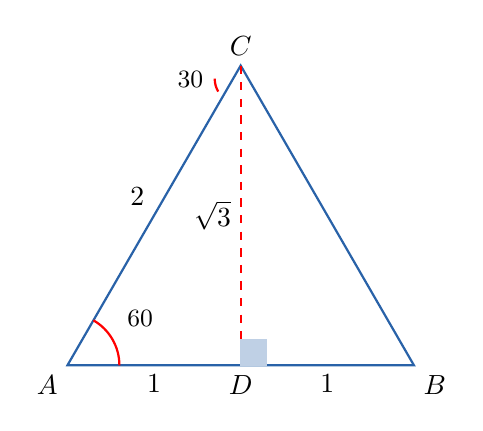
\begin{tikzpicture}[scale=1.1]
  % 等边三角形
  \coordinate (A) at (0,0);
  \coordinate (B) at (4,0);
  \coordinate (C) at (2,3.46);
  \coordinate (D) at (2,0);
  \draw[thick,mainblue] (A)--(B)--(C)--cycle;
  \draw[thick,red,dashed] (C)--(D);
  \node[below left] at (A) {$A$};
  \node[below right] at (B) {$B$};
  \node[above] at (C) {$C$};
  \node[below] at (D) {$D$};
  \draw[red,thick] (A) ++(0.6,0) arc(0:60:0.6);
  \node at ($(A)+(33:1)$) {\small $60°$};
  \draw[red,thick] (C) ++(-0.3,-0.15) arc(-180:-150:0.3);
  \node at ($(C)+(-165:0.6)$) {\small $30°$};
  \filldraw[mainblue!30] (2,0.3) rectangle (2.3,0);
  \node[left] at ($(C)!0.5!(D)$) {$\sqrt{3}$};
  \node[below] at ($(A)!0.5!(D)$) {$1$};
  \node[below] at ($(D)!0.5!(B)$) {$1$};
  \node[above left] at ($(A)!0.5!(C)$) {$2$};
\end{tikzpicture}
\end{center}

在含 $30°$ 角的直角三角形中，设短直角边（$30°$ 的对边）为 $1$，斜边为 $2$，
由勾股定理，长直角边 $= \sqrt{2^2-1^2} = \sqrt{3}$。

\[
\sin 30° = \frac{1}{2},\qquad
\cos 30° = \frac{\sqrt{3}}{2},\qquad
\tan 30° = \frac{1}{\sqrt{3}} = \frac{\sqrt{3}}{3}.
\]

\[
\sin 60° = \frac{\sqrt{3}}{2},\qquad
\cos 60° = \frac{1}{2},\qquad
\tan 60° = \sqrt{3}.
\]

\end{knowledgebox}

\bigskip
\begin{center}
\renewcommand{\arraystretch}{2.0}
\begin{tabular}{|c|c|c|c|}
\hline
\textbf{角} & $30°$ & $45°$ & $60°$ \\
\hline
$\sin$ & $\dfrac{1}{2}$ & $\dfrac{\sqrt{2}}{2}$ & $\dfrac{\sqrt{3}}{2}$ \\
\hline
$\cos$ & $\dfrac{\sqrt{3}}{2}$ & $\dfrac{\sqrt{2}}{2}$ & $\dfrac{1}{2}$ \\
\hline
$\tan$ & $\dfrac{\sqrt{3}}{3}$ & $1$ & $\sqrt{3}$ \\
\hline
\end{tabular}
\end{center}

\begin{tipbox}[记忆技巧]
\begin{itemize}[nosep, leftmargin=1.5em]
  \item \textbf{正弦值}：分母都是 $2$，分子依次为 $\sqrt{1}$、$\sqrt{2}$、$\sqrt{3}$，即 $\dfrac{1}{2}$、$\dfrac{\sqrt{2}}{2}$、$\dfrac{\sqrt{3}}{2}$。
  \item \textbf{余弦值}：与正弦\textbf{刚好反过来}（$30°$ 和 $60°$ 互换）。
  \item \textbf{正切值}：$\dfrac{1}{\sqrt{3}}$、$\dfrac{\sqrt{3}}{\sqrt{3}}$、$\dfrac{\sqrt{3}}{1}$，即 $\dfrac{\sqrt{3}}{3}$、$1$、$\sqrt{3}$。
  \item 口诀：\textbf{一、二、三，分母二；正弦递增余弦反；正切根三上下翻。}
\end{itemize}
\end{tipbox}

% ------- 1.3 互余关系 -------
\subsection*{1.3\quad 互余关系}

\begin{knowledgebox}[互余关系公式]
在直角三角形中，$\angle A + \angle B = 90°$，则：
\[
\boxed{\sin A = \cos(90°-A) = \cos B}
\]
\[
\boxed{\cos A = \sin(90°-A) = \sin B}
\]
\[
\boxed{\tan A = \frac{1}{\tan(90°-A)} = \frac{1}{\tan B}}\quad \text{即}\;\tan A \cdot \tan B = 1
\]

\medskip
\textbf{一句话总结：一个锐角的正弦等于它的余角的余弦。}

\medskip
\textbf{直角三角形中的理解：}
\begin{center}
\begin{tikzpicture}[scale=1.2]
  \coordinate (C) at (0,0);
  \coordinate (A) at (0,3.5);
  \coordinate (B) at (4.5,0);
  \draw[thick,mainblue] (A)--(B)--(C)--cycle;
  \filldraw[mainblue!30] (0,0.35) rectangle (0.35,0);
  \node[above left] at (A) {$A$};
  \node[below right] at (B) {$B$};
  \node[below left] at (C) {$C\;(90°)$};
  \node[left] at ($(A)!0.5!(C)$) {$a$};
  \node[below] at ($(B)!0.5!(C)$) {$b$};
  \node[above right] at ($(A)!0.5!(B)$) {$c$};
  \node at ($(C)!0.65!(A)$) [left] {\small $\sin A = \frac{a}{c}$};
  \node at ($(C)!0.65!(B)$) [below] {\small $\sin B = \frac{b}{c}$};
  \node at (2.8,1.3) {\small $\sin A = \cos B$};
  \node at (2.8,0.8) {\small 因为 $\angle A$ 的对边 $a$};
  \node at (2.8,0.4) {\small 就是 $\angle B$ 的邻边};
\end{tikzpicture}
\end{center}
\end{knowledgebox}

% ------- 1.4 同角三角函数关系（高中预习）-------
\subsection*{1.4\quad 同角三角函数关系（高中预习）}

\begin{knowledgebox}[两个重要的同角关系]
\textbf{关系一：} $\sin^2 A + \cos^2 A = 1$（勾股定理的三角函数形式）

\textbf{推导：}
\[
\sin^2 A + \cos^2 A = \left(\frac{a}{c}\right)^2 + \left(\frac{b}{c}\right)^2 = \frac{a^2+b^2}{c^2} = \frac{c^2}{c^2} = 1
\]

\textbf{关系二：} $\tan A = \dfrac{\sin A}{\cos A}$

\textbf{推导：}
\[
\frac{\sin A}{\cos A} = \frac{a/c}{b/c} = \frac{a}{b} = \tan A
\]

\medskip
这两个公式在高中三角函数中使用极其频繁，务必理解并记住！
\end{knowledgebox}

\begin{tipbox}[公式应用举例]
已知 $\sin A = \dfrac{3}{5}$，可以求出 $\cos A$ 和 $\tan A$：

由 $\sin^2 A + \cos^2 A = 1$：
\[
\cos^2 A = 1 - \sin^2 A = 1 - \frac{9}{25} = \frac{16}{25} \implies \cos A = \frac{4}{5}
\]
\[
\tan A = \frac{\sin A}{\cos A} = \frac{3/5}{4/5} = \frac{3}{4}
\]
\end{tipbox}

% ------- 1.5 解直角三角形 -------
\subsection*{1.5\quad 解直角三角形}

\begin{knowledgebox}[解直角三角形的方法]
\textbf{解直角三角形}：在直角三角形中，由已知元素求出所有未知元素。

直角三角形有 $5$ 个基本元素：$3$ 条边和 $2$ 个锐角（直角已知）。\textbf{已知其中 $2$ 个独立元素（至少含一条边），即可求出其余 $3$ 个。}

\medskip
\textbf{三大关系：}
\begin{enumerate}[nosep, leftmargin=2em]
  \item \textbf{角角关系}：$\angle A + \angle B = 90°$
  \item \textbf{边边关系}（勾股定理）：$a^2 + b^2 = c^2$
  \item \textbf{边角关系}：$\sin A = \dfrac{a}{c}$，$\cos A = \dfrac{b}{c}$，$\tan A = \dfrac{a}{b}$
\end{enumerate}

\medskip
\textbf{选公式口诀}：有斜（斜边）用正弦或余弦，无斜用正切。
\end{knowledgebox}

% ------- 1.6 仰角、俯角、坡度、方向角 -------
\subsection*{1.6\quad 仰角、俯角、坡度与方向角}

\begin{knowledgebox}[仰角与俯角]
\textbf{仰角}：从低处观测高处目标时，视线与水平线的夹角（在水平线上方）。

\textbf{俯角}：从高处观测低处目标时，视线与水平线的夹角（在水平线下方）。

\begin{center}
\begin{tikzpicture}[scale=0.85]
  % 观测点
  \filldraw (0,0) circle(2.5pt);
  % 水平线
  \draw[thick,gray] (-1.5,0)--(6.5,0);
  \node[left] at (-1.5,0) {\small 水平线};
  % 仰角
  \draw[thick,blue] (0,0)--(4.5,4.5);
  \draw[blue,thick] (0,0) ++(1.3,0) arc(0:45:1.3);
  \node at ($(0,0)+(25:1.7)$) {\textcolor{blue}{\small 仰角}};
  \node[right] at (4.5,4.5) {\small 目标（上方）};
  % 俯角
  \draw[thick,red] (0,0)--(4.5,-3.4);
  \draw[red,thick] (0,0) ++(1.3,0) arc(0:-37:1.3);
  \node at ($(0,0)+(-20:1.7)$) {\textcolor{red}{\small 俯角}};
  \node[right] at (4.5,-3.4) {\small 目标（下方）};
\end{tikzpicture}
\end{center}

\textbf{关键：}仰角和俯角都是视线与\textbf{水平线}的夹角，不是与地面的夹角。
\end{knowledgebox}

\begin{knowledgebox}[坡度（坡比）]
\textbf{坡度}：坡面的铅直高度 $h$ 与水平宽度 $l$ 的比值，记作 $i$：
\[
\boxed{i = \frac{h}{l} = \tan\alpha}
\]
其中 $\alpha$ 是坡面与水平面的夹角（\textbf{坡角}）。

\begin{center}
\begin{tikzpicture}[scale=0.75]
  \coordinate (A) at (0,0);
  \coordinate (B) at (9,0);
  \coordinate (C) at (9,3.5);
  \draw[thick,mainblue] (A)--(C);
  \draw[thick,gray] (A)--(B);
  \draw[dashed] (C)--(B);
  \filldraw[mainblue!30] (9,0.35) rectangle (8.65,0);
  \node[below] at ($(A)!0.5!(B)$) {\small 水平距离 $l$};
  \node[right] at ($(B)!0.5!(C)$) {\small 高度 $h$};
  \node[above left] at ($(A)!0.5!(C)$) {\small 坡面};
  \draw[red,thick] (A) ++(1.1,0) arc(0:21.3:1.1);
  \node at ($(A)+(12:1.5)$) {\small 坡角 $\alpha$};
\end{tikzpicture}
\end{center}

例如：坡度 $i = 1:2$ 表示每水平前进 $2$ 米，高度上升 $1$ 米，此时 $\tan\alpha = \dfrac{1}{2}$。
\end{knowledgebox}

\begin{knowledgebox}[方向角]
\textbf{方向角}：以正北或正南方向为基准，向东或向西偏转的角度。

\begin{center}
\begin{tikzpicture}[scale=0.9]
  \draw[thick,->,gray] (0,-0.5)--(0,4.5) node[above]{\small 北(N)};
  \draw[thick,->,gray] (0,0)--(4.5,0) node[right]{\small 东(E)};
  \draw[thick,->,gray] (0,0)--(0,-3.5) node[below]{\small 南(S)};
  \draw[thick,->,gray] (0,0)--(-3.5,0) node[left]{\small 西(W)};
  \filldraw (0,0) circle(2.5pt);
  % 北偏东
  \draw[thick,blue] (0,0)--(3,3.46);
  \draw[blue,thick] (0,0) ++(0.8,0) arc(0:49:0.8);
  \node at ($(0,0)+(27:1.2)$) {\textcolor{blue}{\small 北偏东}};
  % 北偏西
  \draw[thick,red] (0,0)--(-2,3.46);
  \draw[red,thick] (0,0) ++(0,0.8) arc(90:120:0.8);
  \node at ($(0,0)+(107:1.2)$) {\textcolor{red}{\small 北偏西}};
\end{tikzpicture}
\end{center}

\textbf{常见说法：}
\begin{itemize}[nosep, leftmargin=1.5em]
  \item "北偏东 $30°$"：从正北方向顺时针转 $30°$
  \item "南偏西 $45°$"：从正南方向向西（逆时针）转 $45°$
  \item "北偏东"和"东偏北"是\textbf{不同的}方向！
\end{itemize}
\end{knowledgebox}

% ============================================================
%  第二部分：例题精讲
% ============================================================
\section*{\textcolor{examorange}{二、例题精讲}}

% --- 例题1 ---
\begin{examplebox}[【例题1】基础求值——已知两边求三角函数]
在 $\text{Rt}\triangle ABC$ 中，$\angle C=90°$，$a=6$，$b=8$，求 $\sin A$、$\cos A$、$\tan A$。
\end{examplebox}

\textbf{解：}

第一步：由勾股定理求斜边：
\[
c = \sqrt{a^2+b^2} = \sqrt{36+64} = \sqrt{100} = 10
\]

第二步：利用定义求三角函数值：
\[
\sin A = \frac{a}{c} = \frac{6}{10} = \boxed{\frac{3}{5}},\qquad
\cos A = \frac{b}{c} = \frac{8}{10} = \boxed{\frac{4}{5}},\qquad
\tan A = \frac{a}{b} = \frac{6}{8} = \boxed{\frac{3}{4}}
\]

\begin{tipbox}[方法小结]
已知两边求三角函数的步骤：先用勾股定理求第三边，再用定义求值。\\
\textbf{验算技巧}：检查 $\sin^2 A + \cos^2 A = \left(\frac{3}{5}\right)^2+\left(\frac{4}{5}\right)^2 = \frac{9+16}{25}=1$。\checkmark
\end{tipbox}

% --- 例题2 ---
\begin{examplebox}[【例题2】特殊角的混合计算]
求值：$\sin^2 30° + \cos^2 45° + \tan 60° \cdot \cos 30°$。
\end{examplebox}

\textbf{解：}

逐项代入特殊角的值：
\begin{align*}
\sin^2 30° + \cos^2 45° + \tan 60° \cdot \cos 30°
&= \left(\frac{1}{2}\right)^2 + \left(\frac{\sqrt{2}}{2}\right)^2 + \sqrt{3} \cdot \frac{\sqrt{3}}{2} \\[6pt]
&= \frac{1}{4} + \frac{2}{4} + \frac{3}{2} \\[6pt]
&= \frac{1}{4} + \frac{2}{4} + \frac{6}{4} \\[6pt]
&= \boxed{\frac{9}{4}}
\end{align*}

\begin{warnbox}[计算提醒]
\begin{itemize}[nosep, leftmargin=1.5em]
  \item $\sin^2 30°$ 表示 $(\sin 30°)^2$，不是 $\sin(30°^2)$！
  \item $\tan 60° \cdot \cos 30° = \sqrt{3} \times \dfrac{\sqrt{3}}{2} = \dfrac{3}{2}$，注意 $\sqrt{3}\times\sqrt{3}=3$。
\end{itemize}
\end{warnbox}

% --- 例题3 ---
\begin{examplebox}[【例题3】解直角三角形——已知一角一边]
在 $\text{Rt}\triangle ABC$ 中，$\angle C=90°$，$\angle A=30°$，$a=6$，解这个直角三角形。
\end{examplebox}

\textbf{解：}

\begin{itemize}[nosep, leftmargin=2em]
  \item \textbf{求 $\angle B$}：$\angle B = 90° - \angle A = 90° - 30° = 60°$。
  \item \textbf{求 $b$}：$\tan A = \dfrac{a}{b}$，所以 $b = \dfrac{a}{\tan A} = \dfrac{6}{\tan 30°} = \dfrac{6}{\frac{\sqrt{3}}{3}} = \dfrac{6\times 3}{\sqrt{3}} = \dfrac{18}{\sqrt{3}} = 6\sqrt{3}$。
  \item \textbf{求 $c$}：$\sin A = \dfrac{a}{c}$，所以 $c = \dfrac{a}{\sin A} = \dfrac{6}{\sin 30°} = \dfrac{6}{\frac{1}{2}} = 12$。
  \item \textbf{验证}：$a^2+b^2 = 36+108 = 144 = 12^2 = c^2$。\checkmark
\end{itemize}

结论：$\angle B=60°$，$b=6\sqrt{3}$，$c=12$。

% --- 例题4 ---
\begin{examplebox}[【例题4】互余关系的应用]
在 $\text{Rt}\triangle ABC$ 中，$\angle C=90°$，$\sin A = \dfrac{5}{13}$，求 $\cos B$ 和 $\tan B$。
\end{examplebox}

\textbf{解：}

\textbf{方法一（互余关系）：}

因为 $\angle A + \angle B = 90°$，所以：
\[
\cos B = \sin A = \boxed{\frac{5}{13}}
\]

\textbf{方法二（设参数法求 $\tan B$）：}

由 $\sin A = \dfrac{a}{c} = \dfrac{5}{13}$，设 $a = 5k$，$c = 13k$。

由勾股定理：$b = \sqrt{c^2-a^2} = \sqrt{169k^2-25k^2} = 12k$。

\[
\tan B = \frac{b}{a} = \frac{12k}{5k} = \boxed{\frac{12}{5}}
\]

\begin{tipbox}[方法小结]
已知一个角的正弦值求其他三角函数值：\\
利用"设 $k$"的方法，将边长用含 $k$ 的式子表示，最后 $k$ 会消掉。\\
也可以用同角关系：$\cos A = \sqrt{1-\sin^2 A} = \sqrt{1-\frac{25}{169}} = \frac{12}{13}$，再求 $\tan A = \frac{5}{12}$，从而 $\tan B = \frac{1}{\tan A} = \frac{12}{5}$。
\end{tipbox}

% --- 例题5 ---
\begin{examplebox}[【例题5】特殊角计算——化简求值]
求值：$\dfrac{\tan 45° - \sin 30°}{1 + \cos 60°} + \sin 60° \cdot \tan 60°$。
\end{examplebox}

\textbf{解：}

\begin{align*}
\text{原式} &= \frac{1 - \dfrac{1}{2}}{1 + \dfrac{1}{2}} + \frac{\sqrt{3}}{2} \times \sqrt{3} \\[8pt]
&= \frac{\dfrac{1}{2}}{\dfrac{3}{2}} + \frac{3}{2} \\[8pt]
&= \frac{1}{3} + \frac{3}{2} \\[8pt]
&= \frac{2}{6} + \frac{9}{6} \\[8pt]
&= \boxed{\frac{11}{6}}
\end{align*}

% --- 例题6 ---
\begin{examplebox}[【例题6】同角关系证明——$\sin^2 A + \cos^2 A = 1$]
在 $\text{Rt}\triangle ABC$ 中，$\angle C=90°$，求证：$\sin^2 A + \cos^2 A = 1$。
\end{examplebox}

\textbf{证明：}

设 $\angle A$ 的对边为 $a$，邻边为 $b$，斜边为 $c$。

\[
\sin^2 A + \cos^2 A = \left(\frac{a}{c}\right)^2 + \left(\frac{b}{c}\right)^2 = \frac{a^2}{c^2} + \frac{b^2}{c^2} = \frac{a^2+b^2}{c^2}
\]

由勾股定理，$a^2 + b^2 = c^2$，代入得：
\[
\frac{a^2+b^2}{c^2} = \frac{c^2}{c^2} = 1
\]

所以 $\sin^2 A + \cos^2 A = 1$。\qed

\begin{tipbox}[公式的意义]
这个公式叫\textbf{勾股恒等式}，它是勾股定理的三角函数表达形式。\\
在高中，这个公式对\textbf{任意角}都成立，是最基本的三角恒等式之一。
\end{tipbox}

% --- 例题7 ---
\begin{examplebox}[【例题7】方向角与航行问题]
一艘船从 $A$ 港出发，沿北偏东 $60°$ 方向航行 $40$ 海里到达 $B$ 港，再从 $B$ 港沿北偏西 $30°$ 方向航行 $30$ 海里到达 $C$ 港。求 $A$、$C$ 两港之间的距离。

\medskip
\begin{center}
\begin{tikzpicture}[scale=0.42]
  \draw[thick,gray,->] (0,0)--(0,9) node[above]{\small N};
  \draw[thick,gray,->] (0,0)--(8,0) node[right]{\small E};
  \filldraw (0,0) circle(3pt) node[below left]{$A$};
  \coordinate (B) at (5.2,8.66);
  \filldraw (B) circle(3pt) node[right]{$B$};
  \draw[thick,blue] (0,0)--(B) node[midway, right]{\small $40$};
  \draw[blue,thick] (0,0) ++(1,0) arc(0:60:1);
  \node at ($(0,0)+(33:1.4)$) {\small $60°$};
  \coordinate (C) at (0.2,14.66);
  \filldraw (C) circle(3pt) node[above]{$C$};
  \draw[thick,red] (B)--(C) node[midway, right]{\small $30$};
  \draw[red,thick] (B) ++(0,1.3) arc(90:120:1.3);
  \node at (B) ++(107:1.8) {\small $30°$};
  \draw[thick,dashed,mainblue] (0,0)--(C) node[midway, left]{\small $AC$};
\end{tikzpicture}
\end{center}
\end{examplebox}

\textbf{解：}

分析方向角：$AB$ 方向为"北偏东 $60°$"（从正北顺时针 $60°$），$BC$ 方向为"北偏西 $30°$"（从正北逆时针 $30°$）。

$\angle ABC$ 的计算：$\angle ABC = 180° - 60° - 30° = 90°$。

所以在 $\text{Rt}\triangle ABC$ 中，$AB = 40$，$BC = 30$。

由勾股定理：
\[
AC = \sqrt{AB^2+BC^2} = \sqrt{40^2+30^2} = \sqrt{1600+900} = \sqrt{2500} = \boxed{50 \text{ 海里}}
\]

% --- 例题8 ---
\begin{examplebox}[【例题8】综合应用——利用同角关系求值]
已知 $\sin A = \dfrac{3}{5}$，$A$ 为锐角，求 $\cos A$ 和 $\tan A$。
\end{examplebox}

\textbf{解：}

\textbf{方法一（勾股恒等式）：}

由 $\sin^2 A + \cos^2 A = 1$：
\[
\cos^2 A = 1 - \sin^2 A = 1 - \left(\frac{3}{5}\right)^2 = 1 - \frac{9}{25} = \frac{16}{25}
\]

因为 $A$ 为锐角，$\cos A > 0$，所以 $\cos A = \dfrac{4}{5}$。

\[
\tan A = \frac{\sin A}{\cos A} = \frac{3/5}{4/5} = \frac{3}{4}
\]

\textbf{方法二（设参数法）：}

由 $\sin A = \dfrac{a}{c} = \dfrac{3}{5}$，设 $a = 3$，$c = 5$。

$b = \sqrt{c^2-a^2} = \sqrt{25-9} = 4$。

$\cos A = \dfrac{b}{c} = \dfrac{4}{5}$，$\tan A = \dfrac{a}{b} = \dfrac{3}{4}$。

结论：$\cos A = \boxed{\dfrac{4}{5}}$，$\tan A = \boxed{\dfrac{3}{4}}$。

% ============================================================
%  第三部分：应用题
% ============================================================
\section*{\textcolor{apppurple}{三、应用题}}

% --- 应用1 ---
\begin{appbox}[【应用1】测量楼高——仰角问题]
小明在距离一栋大楼底部 $30\,\text{m}$ 的 $A$ 点处，测得楼顶 $C$ 的仰角为 $30°$。已知小明的眼睛距地面 $1.5\,\text{m}$，求大楼的高度（精确到 $0.1\,\text{m}$）。

\medskip
\begin{center}
\begin{tikzpicture}[scale=0.55]
  \fill[lightgray!20] (-1,0) rectangle (13,-0.3);
  \draw[thick] (-1,0)--(13,0);
  \draw[very thick,mainblue] (10,0)--(10,8);
  \draw[thick,blue] (1,0)--(1,1.5);
  \filldraw[blue] (1,1.5) circle(2.5pt);
  \draw[dashed,red] (1,1.5)--(10,8);
  \draw[thick,gray] (1,1.5)--(10,1.5);
  \draw[red,thick] (1,1.5) ++(1.5,0) arc(0:36.9:1.5);
  \node at (1,1.5) ++(20:2) {\small $30°$};
  \node[left] at (1,0.75) {\small $1.5\,$m};
  \draw[<->] (1,-0.5)--(10,-0.5);
  \node at (5.5,-0.8) {\small $30\,$m};
  \node[left] at (1,0) {\small $A$};
  \node[above] at (10,8) {\small $C$（楼顶）};
  \node at (10,-0.3) {\small $B$};
\end{tikzpicture}
\end{center}
\end{appbox}

\textbf{解：}

如图，设 $C$ 到小明眼睛水平线的高度为 $h$。

在直角三角形中：
\[
\tan 30° = \frac{h}{30},\quad h = 30\tan 30° = 30 \times \frac{\sqrt{3}}{3} = 10\sqrt{3} \approx 17.32\,\text{m}
\]

大楼总高 $= h + 1.5 = 17.32 + 1.5 = \boxed{18.8\,\text{m}}$。

\begin{warnbox}[易错提醒]
仰角问题中，总高度 $=$ 眼睛到目标的垂直高度 $+$ 眼睛离地高度。\\
不要忘记加上观测者眼睛的高度！
\end{warnbox}

% --- 应用2 ---
\begin{appbox}[【应用2】航行问题——方向角综合]
一艘轮船从 $A$ 港出发，沿北偏东 $45°$ 方向航行 $20\sqrt{2}$ 海里到达 $B$ 港，再从 $B$ 港沿正东方向航行 $20$ 海里到达 $C$ 港。求：
（1）$B$ 港在 $A$ 港的什么位置（用方向角表示）；
（2）$C$ 港在 $A$ 港的什么方向，$A$、$C$ 两港相距多远？

\medskip
\begin{center}
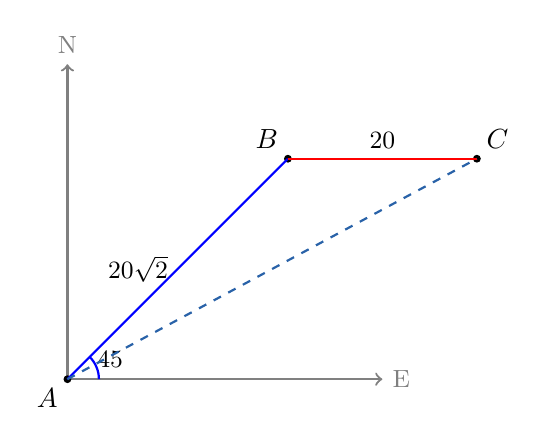
\begin{tikzpicture}[scale=0.4]
  \draw[thick,gray,->] (0,0)--(0,10) node[above]{\small N};
  \draw[thick,gray,->] (0,0)--(10,0) node[right]{\small E};
  \filldraw (0,0) circle(3pt) node[below left]{$A$};
  \coordinate (B) at (7,7);
  \filldraw (B) circle(3pt) node[above left]{$B$};
  \draw[thick,blue] (0,0)--(B);
  \draw[blue,thick] (0,0) ++(1,0) arc(0:45:1);
  \node at ($(0,0)+(25:1.5)$) {\small $45°$};
  \coordinate (C) at (13,7);
  \filldraw (C) circle(3pt) node[above right]{$C$};
  \draw[thick,red] (B)--(C);
  \draw[thick,dashed,mainblue] (0,0)--(C);
  \node[above] at ($(0,0)!0.5!(B)$) [left] {\small $20\sqrt{2}$};
  \node[above] at ($(B)!0.5!(C)$) {\small $20$};
\end{tikzpicture}
\end{center}
\end{appbox}

\textbf{解：}

（1）$B$ 港在 $A$ 港的\textbf{北偏东 $45°$}方向，距离 $20\sqrt{2}$ 海里。

（2）建立辅助直角三角形。过 $B$ 作 $BD \perp$ 东西方向线（$D$ 在 $A$ 的正东方向上）。

由方向角，$AB$ 为北偏东 $45°$，所以 $\triangle ABD$ 是等腰直角三角形：
\[
AD = AB \cdot \sin 45° = 20\sqrt{2} \times \frac{\sqrt{2}}{2} = 20,\qquad
BD = AB \cdot \cos 45° = 20\sqrt{2} \times \frac{\sqrt{2}}{2} = 20
\]

$BC$ 向正东，所以 $DC = AD + BC = 20 + 20 = 40$。

在 $\text{Rt}\triangle ADC$ 中：
\[
AC = \sqrt{AD^2+DC^2} = \sqrt{20^2+40^2} = \sqrt{400+1600} = \sqrt{2000} = 20\sqrt{5} \approx 44.7 \text{ 海里}
\]

方向角：$\tan(\angle DAC) = \dfrac{DC}{BD} = \dfrac{40}{20} = 2$，$\angle DAC \approx 63.4°$。

所以 $C$ 港在 $A$ 港的\textbf{北偏东约 $63.4°$}方向，相距约 $\boxed{44.7 \text{ 海里}}$。

% --- 应用3 ---
\begin{appbox}[【应用3】坡度计算]
一段斜坡路面的坡度为 $1:\sqrt{3}$。一辆汽车沿斜坡向上行驶了 $200\,\text{m}$，求：
（1）坡角是多少度？
（2）汽车上升了多少米？水平前进了多少米？

\medskip
\begin{center}
\begin{tikzpicture}[scale=0.55]
  \coordinate (A) at (0,0);
  \coordinate (B) at (10,0);
  \coordinate (C) at (10,4);
  \draw[thick,mainblue,line width=1.5pt] (A)--(C);
  \draw[thick,gray] (A)--(B);
  \draw[dashed] (C)--(B);
  \filldraw[mainblue!30] (10,0.35) rectangle (9.65,0);
  \node[below] at ($(A)!0.5!(B)$) {\small 水平距离 $l$};
  \node[right] at ($(B)!0.5!(C)$) {\small 高度 $h$};
  \node[above left] at ($(A)!0.5!(C)$) {\small 斜坡 $200\,$m};
  \draw[red,thick] (A) ++(1.1,0) arc(0:21.8:1.1);
  \node at ($(A)+(12:1.5)$) {\small 坡角 $\alpha$};
\end{tikzpicture}
\end{center}
\end{appbox}

\textbf{解：}

（1）坡度 $i = \dfrac{h}{l} = \dfrac{1}{\sqrt{3}} = \tan\alpha$。

由特殊角值可知 $\tan 30° = \dfrac{1}{\sqrt{3}}$，所以坡角 $\alpha = \boxed{30°}$。

（2）
\begin{itemize}[nosep, leftmargin=2em]
  \item 上升高度：$h = 200 \times \sin 30° = 200 \times \dfrac{1}{2} = \boxed{100\,\text{m}}$。
  \item 水平距离：$l = 200 \times \cos 30° = 200 \times \dfrac{\sqrt{3}}{2} = \boxed{100\sqrt{3} \approx 173.2\,\text{m}}$。
\end{itemize}

% ============================================================
%  第四部分：课堂练习
% ============================================================
\section*{\textcolor{tipgreen}{四、课堂练习}}

\begin{enumerate}[leftmargin=2em, itemsep=10pt]

  \item 在 $\text{Rt}\triangle ABC$ 中，$\angle C=90°$，$a=5$，$c=13$，求 $\sin A$、$\cos A$、$\tan A$。

  \item 求值：$\sin 60° \cdot \cos 30° + \tan 45° - \sin^2 45°$。

  \item 在 $\text{Rt}\triangle ABC$ 中，$\angle C=90°$，$\cos A = \dfrac{4}{5}$，求 $\sin A$ 和 $\tan A$。

  \item 在 $\text{Rt}\triangle ABC$ 中，$\angle C=90°$，$\angle A=60°$，$c=10$，求 $a$ 和 $b$。

  \item 在 $\text{Rt}\triangle ABC$ 中，$\angle C=90°$，$a=2\sqrt{3}$，$b=2$，求 $\angle A$ 和 $\angle B$。

  \item 已知 $\tan A = \dfrac{3}{4}$，$A$ 为锐角，求 $\sin A$ 和 $\cos A$。

  \item 一棵大树被风吹断，树顶着地于 $C$ 点，$C$ 点距树根 $A$ 的水平距离为 $8\,\text{m}$，折断部分 $BC$ 与地面的夹角为 $30°$，求大树原来的高度。

  \item 从 $20\,\text{m}$ 高的楼顶 $A$ 处测得对面一棵树顶 $C$ 的俯角为 $30°$，又测得树底 $D$ 的俯角为 $45°$。求树高 $CD$（精确到 $0.1\,\text{m}$）。

\end{enumerate}

\vspace{10pt}
\begin{knowledgebox}[参考答案]

\begin{enumerate}[leftmargin=2em, itemsep=6pt]

  \item $b = \sqrt{c^2-a^2} = \sqrt{169-25} = 12$。
  \[
  \sin A = \frac{5}{13},\quad \cos A = \frac{12}{13},\quad \tan A = \frac{5}{12}.
  \]

  \item $\sin 60° \cdot \cos 30° + \tan 45° - \sin^2 45°
  = \dfrac{\sqrt{3}}{2} \cdot \dfrac{\sqrt{3}}{2} + 1 - \left(\dfrac{\sqrt{2}}{2}\right)^2
  = \dfrac{3}{4} + 1 - \dfrac{1}{2}
  = \boxed{\dfrac{5}{4}}$。

  \item $\cos A = \dfrac{4}{5}$，设 $b=4$，$c=5$，则 $a = \sqrt{25-16} = 3$。\quad $\sin A = \dfrac{3}{5}$，$\tan A = \dfrac{3}{4}$。

  \item $\angle B = 90°-60° = 30°$。

  $a = c\sin 60° = 10 \times \dfrac{\sqrt{3}}{2} = \boxed{5\sqrt{3}}$，\quad $b = c\cos 60° = 10 \times \dfrac{1}{2} = \boxed{5}$。

  \item $\tan A = \dfrac{a}{b} = \dfrac{2\sqrt{3}}{2} = \sqrt{3}$，所以 $\angle A = 60°$，$\angle B = 30°$。

  \item 由 $\tan A = \dfrac{3}{4}$，设 $a=3$，$b=4$，则 $c=\sqrt{9+16}=5$。\\
  $\sin A = \dfrac{3}{5}$，$\cos A = \dfrac{4}{5}$。

  \item 设断点 $B$ 高 $h$，则 $\tan 30° = \dfrac{h}{8}$，$h = 8\tan 30° = \dfrac{8\sqrt{3}}{3}$。

  折断部分 $BC = \dfrac{8}{\cos 30°} = \dfrac{16\sqrt{3}}{3}$。

  原高 $= h + BC = \dfrac{8\sqrt{3}}{3} + \dfrac{16\sqrt{3}}{3} = 8\sqrt{3} \approx \boxed{13.9\,\text{m}}$。

  \item 由俯角 $45°$：$A$ 到树的水平距离 $d = 20\,\text{m}$。

  由俯角 $30°$：$\tan 30° = \dfrac{20-h_C}{d}$（$h_C$ 为树顶离地高）。

  实际上：$\tan 30° = \dfrac{20-h_C}{20}$，$20-h_C = \dfrac{20\sqrt{3}}{3}$。

  树顶高 $h_C = 20 - \dfrac{20\sqrt{3}}{3}$，树底高 $= 0$（在地面）。

  树高 $CD = 20 - \dfrac{20\sqrt{3}}{3} = \dfrac{60-20\sqrt{3}}{3} \approx \boxed{8.5\,\text{m}}$。

\end{enumerate}
\end{knowledgebox}

\vfill
\begin{center}
\small\textcolor{gray}{三角函数是高中数学最重要的章节之一，初中基础必须扎实。多练多算，熟能生巧！}
\end{center}

\end{document}
